\graphicspath{{./chapters/04-physical_design/figures/}}

\chapter{Physical design}
\label{chap:physical_design}
The physical design has been performed using \textit{Innovus 17.11} starting
from the post-synthesis netlist and sdc file generated by the \textit{Standard
synthesis} described in \ref{subsec:std_syn}.

\section{Results}
Following paragraphs summarize results obtained by the physical design process.
\paragraph{Layout view} \mbox{} \\
\begin{figure}[H]
	\centering
	\frame{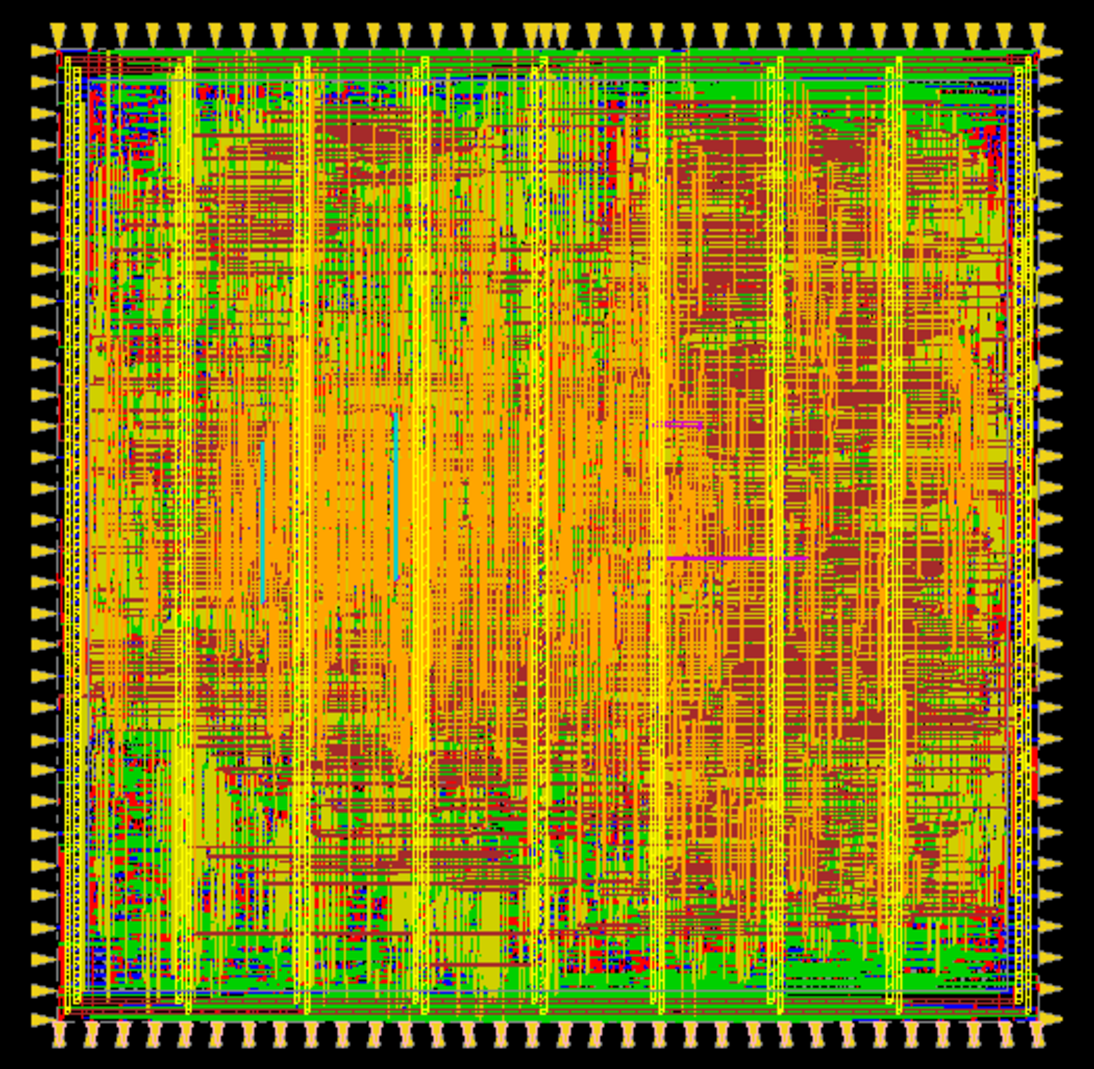
\includegraphics[width=.5\textwidth]{screen_capture}}
	\label{fig:layout}
	\caption{The DLXY physical layout.}
\end{figure}

\paragraph{Timing reports} \mbox{} \\
\lstset{
	basicstyle=\tiny,
	frame=single,
	breaklines=true
}
\lstinputlisting{chapters/04-physical_design/files/dlx_postRoute.summary}
\lstinputlisting{chapters/04-physical_design/files/dlx_postRoute_hold.summary}

\paragraph{Gate count report} \mbox{} \\
\lstinputlisting{chapters/04-physical_design/files/dlx.gateCount}

\section{Comparison with synthesis results}
After the physical design process there is no violating path (neither for the
setup not for the hold time) and the total area value is very similar to the one
reported by the synthesizer: this means that the physical design results are
coherent with the synthesis.

